\section{Computational Experience}
\label{sec:Experimentalwork}

In this section, we present the evaluation
of the proposed algorithms.
All methods were coded in Python version 3.10.0 and the algebraic modeling language Pyomo version 6.6.1 using IBM(R) ILOG(R) CPLEX(R) version 22.1.0.0 as the optimization solver. Tests were carried out in a 64-bit platform with 64 GB of RAM and 2.50 GHz Intel(R) i7(R) 11700 CPU, 65W, on a Linux Ubuntu version 20.0 operating system. 

For all tests the relative optimality gap (ROG) was computed as follows:
%
\begin{equation}
\label{ec:gap}
\text{ROG} = \frac{|LowBound-z\_best|}{((1 \times 10^{-10})+|z\_best|)} \cdot 100 \% \nonumber
\end{equation}
%
where $LowBound$ corresponds to the largest lower (dual) bound obtained by the branch-and-bound solver and $z\_best$, to the best feasible integer solution found by the corresponding method.
%def igap(LB,UB):
%    return abs( LB - UB ) / ( 1e-10 + abs(UB) )    

\subsection{Description of test instances}  
A total of 83 instances, divided into three main subsets (see Table~\ref{tab:instancesKazarlis}), were used to evaluate the proposed methods. The first subset, x7day\_small, consists of 20 instances (10 from \citet{Morales-Espania2013} and 10 derived from an eight-generator dataset proposed by \citet{Ostrowski2012}); while the second (x7day\_medium) and third (x7day\_large)  subsets include 33 and 30 instances, respectively, constructed by gradually increasing the number of generators and randomly combining them to enhance complexity, based on data from \citet{Ostrowski2012}. The planning horizon for all the sets is composed of 168 periods, equivalent to seven days. 
\textcolor{blue}{The configuration of each instance can be consulted in Appendix \ref{app:appD}}

\begin{table}[htb]
\centering
\caption{Description of test instances.}\label{tab:instancesKazarlis}
\begin{tabular}{lrrr}\toprule
Group &Instances &Generators &Instances  \\\cmidrule{1-4}
x7day\_small &20 &28-81 &061-070, 101-110    \\
x7day\_medium &33 &85-156 &071-073, 111-140  \\
x7day\_large &30 &165-405 &074-080, 141-163 \\
\bottomrule
\end{tabular}
\end{table}


The demand profile for each instance, shown in Table \ref{tab:Load}, is obtained by multiplying the demand profile and the sum of the maximum capacity of all generators. A reduction factor of 80\% on a weekday is applied to calculate the weekend demand. The spinning reserve requirement is 5\% of the hourly power demand, except for the 19 instances derived from \citet{Morales-Espania2013} (061--080, excluding 062), which use 10\%.

\begin{table}[H]
\centering
\caption{Load demand profile (\% of total capacity).}\label{tab:Load}
\scriptsize
\begin{tabular}{lrrrrrrrrrrrrr}\toprule
hour &1 &2 &3 &4 &5 &6 &7 &8 &9 &10 &11 &12 \\
demand &71\% &65\% &62\% &60\% &58\% &58\% &60\% &64\% &73\% &80\% &82\% &83\% \\\cmidrule{1-13}
hour &13 &14 &15 &16 &17 &18 &19 &20 &21 &22 &23 &24 \\
demand &82\% &80\% &79\% &79\% &83\% &91\% &90\% &88\% &85\% &84\% &79\% &74\% \\
\bottomrule
\end{tabular}
\end{table}



%%%%%%%%%%%%%%%%%%%%%%%%%%%%%%%%%%%%5
%%%%%%%%%%%%%%%%%%%%%%%%%%%%%%%%%%%%5
%%%%%%%%%%%%%%%%%%%%%%%%%%%%%%%%%%%%%
\subsection{Comparison of constructive methods}
\label{section:Test1}

The goal of this first experiment is to evaluate
the proposed construction heuristic, HARDUC.
To this end, we compare HARDUC, HGPS \citep{Harjunkoski2021}, and the best solution found
by CPLEX (CBS, for CPLEX Best Solution) on all the instances.
%
 CPLEX algorithmic parameters such as \textit{emphasis\_mip}, \textit{mip\_strategy\_file}, and \textit{mip\_tolerances\_mipgap}, were configured as detailed in Table \ref{tab:parameters_solverMILP1}. The maximum computing time was set to 1200 s.  The table shows the average ROG (AROG) and its standard deviation (ROGSD), as well as the number of feasible solutions (NFS) that the each method successfully found.
%Less than two hours is typically the expected time to resolve it \citep{Santos2020}

\begin{table}[H]
\centering
\caption{Parameters of the solver used as constructive CBS.}
\label{tab:parameters_solverMILP1}
\scriptsize
\begin{tabular}{>{\RaggedRight}p{3.5cm}r>{\RaggedRight}p{6cm}r}\toprule
{Parameter} & {Value} & {Description} \\\cmidrule{1-3}
emphasis\_mip &1 &Emphasize feasibility over optimality \\
mip\_strategy\_file &3 &Node file on disk and compressed \\
mip\_tolerances\_mipgap & $1 \times 10^{-6}$  &Relative tolerance between the best integer and the best lower bound \\
\bottomrule
\end{tabular}
\end{table}


Table \ref{tab:descriptive_constructive} shows the comparison of the obtained results. These results indicate that the proposed HARDUC achieved the lowest AROG among all the sets of instances, indicating solutions closer to optimality than CBS and HGPS. It also obtained the lowest ROGSD, ensuring more stable performance. CBS showed the highest AROG and ROGSD in most of the cases. HGPS performed better than CBS but slightly  worse than HARDUC. In terms of the number of feasible solutions, HARDUC successfully found feasible solutions for all the sets of instances. HGPS identified 20/32/29 feasible solutions for the sets of small-, medium-, and large-scale instances, respectively. Finally, CPLEX found 20 feasible solutions in the x7day\_small group (100\%), 26 out of 33 in the x7day\_medium group (78.7\%), and 18 out of 30 in the x7day\_large group (63.3\%).


\begin{table}[H]\centering
\caption{Comparison of constructive methods.}
\label{tab:descriptive_constructive}
\scriptsize
\scalebox{1}{
\begin{tabular}{lrrr|rrr|rrr}\toprule
&\multicolumn{3}{c}{x7day\_small} &\multicolumn{3}{c}{x7day\_medium} &\multicolumn{3}{c}{x7day\_large} \\\cmidrule{2-10}
Method & AROG   & ROGSD  & NFS & AROG   & ROGSD  & NFS & AROG   & ROGSD  & NFS \\\cmidrule{1-10}
CBS    & 0.0075 & 0.0195 & 20  & 0.0005 & 0.0001 & 26  & 0.0071 & 0.0186 & 18 \\
HGPS   & 0.0013 & 0.0003 & 20  & 0.0010 & 0.0002 & 32  & 0.0009 & 0.0004 & 29 \\
HARDUC & 0.0007 & 0.0002 & 20  & 0.0005 & 0.0001 & 33  & 0.0003 & 0.0000 & 30 \\
\bottomrule
%\multicolumn{10}{l}{\footnotesize * Values are in USD. \citep{Morales-Espania2013}}
\end{tabular}
}
\end{table}



Therefore, HARDUC was chosen to obtain an initial feasible solution for the proposed matheuristics evaluated in the next section since it obtained the best performance.

 %In summary, as the instance size increases, the number of solutions found by other methods decreases for , while the proposed constructive method consistently discovers an initial solution within the specified time constraints.



%%% Analysis of variance moved to appendix

%%%%%%%%%%%%%%%%%%%%%%%%%%%%%%%%%%%%%%%%%%%%%
%%%%%%%%%%%%%%%%%%%%%%%%%%%%%%%%%%%%%%%%%%%%%
%%%%%%%%%%%%%%%%%%%%%%%%%%%%%%%%%%%%%%%%%%%%%
\subsection{Evaluation of metaheuristics performance}
\label{section:Test2}

In the following tests, the proposed methods (KS and the four versions of LB) are evaluated under two different computation times: 4000 s.\ and 7200 s.\ (including the time for obtaining the initial feasible solution). For all LB versions, each iteration has a time limit of 1200 s., except the first
subproblem of the search and each subproblem solved right after a diversification restart, which are
limited to 100 s.\ in order to probe the neighborhood cheaply before committing the remaining budget.


\textcolor{blue}{
%Before presenting the comparison with the off-the-shelf solver, 
It is important to clarify that the proposed matheuristics do not operate independently from the solver. Instead, they work alongside CPLEX, invoking the solver as an exact component repeatedly throughout the search. In this sense, the matheuristics function in tandem with the solver, guiding and accelerating its convergence rather than replacing it. To assess the extent of this synergy, we also include experiments in which the model is solved solely by CPLEX, allowing us to verify whether the combined methods indeed outperform the solver on its own.
}

\color{blue}
%\subsubsection{Comparison with an off-the-shelf solver} 

To establish this baseline, we evaluate the performance of CPLEX when solving the TUCP model \eqref{eq:obj}–\eqref{eq:pp}. Two benchmark methods were considered. In Solver Method 1 (SM1), the TUCP model is solved directly by CPLEX without any warm start. In Solver Method 2 (SM2), an initial feasible solution generated by our constructive heuristic is provided to the solver as a MIP start. For all methods (except SM1), the same initial solution is used to ensure a fair comparison. The specific CPLEX parameters adopted for these experiments are reported in Table~\ref{tab:parameters_solverMILP2}.
\color{black}

%the results obtained by solving model TUCP ( \eqref{eq:obj}-\eqref{eq:pp}) using CPLEX, are analyzed. For this purpose, two versions were considered: SM1 (Solver method 1), in which the model is completely solved by CPLEX, and SM2 (Solver method 1), where an initial feasible solution is given as a staring solution (MIPStart) to the solver. For all methods (except SM1), the same initial solution is considered. Certain parameters used by CPLEX were adjusted as specified in Table \ref{tab:parameters_solverMILP2}.

%The solver parameters for these improvement methods have been tuned to emphasize the search for feasible solutions over the search for optimal solutions \citep{Fischetti2003}.

\begin{table}[H]
\centering
\caption{CPLEX algorithmic parameters for matheuristic evaluation.}
\label{tab:parameters_solverMILP2}
\scriptsize
\begin{tabular}{c>{\RaggedRight}p{3.5cm}r>{\RaggedRight}p{6cm}r}\toprule
Method & {Parameter} & {Value} & {Description} \\\cmidrule{1-4}
\multirow{4}{*}{{SM1}} &emphasis\_mip &1 &Emphasize feasibility over optimality \\
&mip\_strategy\_file &3 &Node file on disk and compressed \\
&mip\_tolerances\_mipgap & $1 \times 10^{-6}$ &Relative tolerance between the best integer and the best lower bound \\
&preprocessing\_symmetry &$-1$ &CPLEX default (automatic symmetry detection) \\
\bottomrule \bottomrule
\multirow{4}{*}{{Remaining}} &emphasis\_mip &1 &Emphasize feasibility over optimality \\
&mip\_strategy\_file &3 &Node file on disk and compressed \\
&mip\_tolerances\_mipgap & $1 \times 10^{-6}$ &Relative tolerance between the best integer and the best lower bound \\
&preprocessing\_symmetry &0 &Turn off symmetry breaking \\
\bottomrule
\end{tabular}
\end{table}

Any CPLEX parameter not listed in Table \ref{tab:parameters_solverMILP2} was left at its default value.

For the relevant criteria specific to each proposed solution method, Table \ref{tab:methods} illustrates how these were applied.

\begin{table}[htpb]
\centering
\small
\caption{Criteria considered for the KS and the LB methods.}\label{tab:methods}
\begin{tabular}{p{1.5cm}ll}\toprule
\multirow{3}{*}{LB1} 
& LBC\tnote{1}~built using dominant variable $u_{g,t}$. \\
& RCL from Harjukovski's rule \citep{Harjunkoski2021}. \\
& Soft-fixing to 90\% of binary support. \\ 
\cmidrule{2-2}
\multirow{2}{*}{LB2} 
& LBC built using dominant variable $u_{g,t}$. \\
& RCL from Harjukovski's rule \citep{Harjunkoski2021}. \\ 
\cmidrule{2-2}
\multirow{1}{*}{LB3} 
& LBC built using dominant variable $u_{g,t}$. \\  
\cmidrule{2-2}
\multirow{3}{*}{LB4} 
& LBC built using dominant variable $u_{g,t}$. \\
& RCL from reduced costs. \\ 
& Soft-fixing to 90\% of binary support. \\ 
\cmidrule{2-2}
\multirow{4}{*}{KS} 
%& The first solution is given by the HARDUC constructive method. \\
& Kernel and buckets are built only with dominant variables $u_{g,t}$. \\
& Number of buckets is calculated by Sturge's rule \citep{Scott2009}. \\
& Buckets are built using the reduced costs from linear relaxation (fixing kernel). \\
\bottomrule
\end{tabular}
\end{table}
%&The buckets are built using the ordered reduced costs fixing the Kernel and solving linear relaxation. \\

Table \ref{tab:descriptive_fused} shows the AROG, the ROGSD, and the NFS obtained for each method considering the set of test instances. As can be seen, on average, increasing the maximum computation time reduce the average ROG and its corresponding standard deviation in most cases. Considering the significant impact that improvements can have, even if they are perceived to be small, we can visualize that by assigning one more hour of optimization (which is still within the time allowed in the real case), we can further improve the solutions obtained when the optimization time is 4000 s.

%limit. However, some medium- (NFS = 26/33) and large-scale (NFS = 28/30) instances were excluded in the 

Our proposed construction heuristic, HARDUC, found feasible solutions for all instances within the time limit. However, some medium- and large-scale instances were excluded in the computations under the 7200 s. \textcolor{blue}{option because the base solver failed to find an initial feasible integer solution at the root node of the branch-and-bound method, so no upper bound was available, although the linear relaxation (lower bound) could be obtained. We point out in Appendix~\ref{app:appD} the instances without an initial integer solution. This issue (failure to find an initial feasible integer solution) has also been reported in previous studies \citep{Cong2015,Knueven2020b,Morales-Espania2015,Wuijts2024} }.

%WRONG!!! option because CPLEX, the base solver, failed to solve the linear programming relaxation at the root node of the branch-and-bound method so that no lower bound was available. !!!



%solve them in 7000 seconds, and therefore statistics for SM! cannot eb computed in those cases. %As the ROG metric depends on the best solution found, these cases were omitted. TENGO DUDAS!!}



\begin{table}[htpb]
\centering
\caption{Performance comparison among all solution methods considering different maximum time limits}
\label{tab:descriptive_fused}
\scriptsize
\begin{tabular}{llrrr|rrr}
\toprule
\cmidrule{2-8}
\multicolumn{1}{c}{Set} &Method &\multicolumn{3}{c}{4000 s} & \multicolumn{3}{c}{7200 s}\\
\cmidrule{3-8}
& & AROG & ROGSD & NFS & AROG & ROGSD & NFS \\
\midrule
 \multirow{7}{*}{x7day\_small} & LB1 &6.65E-4 &2.20E-4 &20 &6.11E-4 &1.82E-4 &20 \\
&LB2 &  6.56E-4 &2.18E-4 &20 &6.22E-4 &2.00E-4 &20 \\
&LB3 &  6.98E-4 &2.44E-4 &20 &6.67E-4 &2.31E-4 &20 \\
&LB4 &  6.60E-4 &2.30E-4 &20 &6.31E-4 &2.06E-4 &20 \\
&KS  &  6.85E-4 &2.63E-4 &20 &6.78E-4 &2.67E-4 &20 \\
&SM1 &  5.79E-4 &1.59E-4 &20 &5.56E-4 &1.59E-4 &20 \\
&SM2 &  6.28E-4 &1.49E-4 &20 &5.81E-4 &1.55E-4 &20 \\
\midrule
\multirow{7}{*}{x7day\_medium} &LB1  &3.74E-4 &9.08E-5 &26 &3.36E-4 &7.25E-5 &26 \\
&LB2  &3.66E-4 &9.49E-5 &26 &3.39E-4 &7.67E-5 &26 \\
&LB3  &3.82E-4 &9.44E-5 &26 &3.50E-4 &6.46E-5 &26 \\
&LB4  &3.76E-4 &9.19E-5 &26 &3.38E-4 &6.91E-5 &26 \\
&KS   &3.10E-4 &7.48E-5 &26 &2.98E-4 &6.73E-5 &26 \\
&SM1  &4.73E-4 &1.18E-4 &26 &3.13E-4 &8.77E-5 &26 \\
&SM2  &3.74E-4 &9.08E-5 &26 &4.45E-4 &1.07E-4 &26 \\
\midrule
\multirow{7}{*}{x7day\_large} & LB1  &2.71E-4 &6.42E-5 &18 &2.47E-4 &5.75E-5 &18 \\
&LB2 &  2.81E-4 &7.17E-5 &18 &2.42E-4 &5.82E-5 &18 \\
&LB3 &  2.91E-4 &7.36E-5 &18 &2.63E-4 &6.44E-5 &18 \\
&LB4 &  2.90E-4 &6.64E-5 &18 &2.54E-4 &6.30E-5 &18 \\
&KS  &  2.25E-4 &3.95E-5 &18 &2.08E-4 &3.82E-5 &18 \\
&SM1 &  3.07E-4 &8.77E-5 &18 &2.72E-4 &7.33E-5 &18 \\
&SM2 &  3.33E-4 &7.79E-5 &18 &3.19E-4 &8.34E-5 &18 \\
\bottomrule
%\multicolumn{8}{l}{\footnotesize * Values are in USD. \citep{Morales-Espania2013}}
\end{tabular}
\end{table}


Finally, the results are also plotted for all methods and each set of instances. A statistical analysis is conducted only for those instances in which the method successfully found a solution. Figures \ref{fig_violinAll_1h_x7day_small}, \ref{fig_violinAll_1h_x7day_medium}, and \ref{fig_violinAll_1h_x7day_large} present the distributions of the relative optimality gap for each method. Each series represents a method, with the horizontal axis indicating the relative optimality gap. The Y-axis represents the density, which is a continuous estimate of the relative frequency. Therefore, the area under the curve must equal 1. The figures show that as instance difficulty increases, the KS and LB methods yield results with significantly lower variance compared to the solver (SM1, SM2). Additionally, the KS and LB methods achieve higher accuracy, with an average relative optimality gap closer to zero than the solver. To assess the significance of these improvements, we conducted statistical tests by analyzing variance and comparing means. 

Similarly, Figures \ref{fig_violinAll_2h_x7day_small}, \ref{fig_violinAll_2h_x7day_medium}, and \ref{fig_violinAll_2h_x7day_large} provide evidence of the relative optimality gap distributions for each method at 7200 s. It can be noticed that, as instance difficulty increases, the KS outperforms the other methods, showing a lower variance and a superior accuracy of AROG.

An analysis of variance (ANOVA) was conducted for each set of instances in both cases. The results reject the null hypothesis of equal means, confirming that at least one method differs significantly from the others. Similar results are obtained when the maximum time limit allowed is 7200 s (see Appendix \ref{app:appB} for details).

%\hl{Caray, los gaps son tan pequenos que tenemos que decir algo donde la escala impacte.  Por ej.}
%\hl{It is important to note that even though the relative optimality gaps are in the order of 1E-4, the dimension of the objective function value is in the order of TENS of billions of dollars, thus, even a small improvement of 0.01\% or 0.001\% is meaningful in practice.  Es cierto esto? UILL - AGREGUE LOS PARRAFOS  DE ABAJO EN AZUL  PARA ACLARAR ESTO: SE ACEPTAN COMENTARIOS/ MEJORAS }


It is important to realize that even very small relative optimality gaps, on the order of 0.01\% or less, can lead to materially different market outcomes. These differences may not significantly affect the total cost, but they can shift unit commitment decisions enough to alter the marginal prices used for market settlements. Since these prices determine generator payments, slight variations can result in economic mismatches and fairness concerns \citep{Johnson1997}.

This sensitivity has been confirmed in several studies, where near-optimal solutions with nearly identical objective values led to significantly different pricing outcomes. As shown by \citet{Sioshansi2008}, small optimality gaps do not necessarily eliminate payment deviations or price volatility. Therefore, reducing the gap (even marginally) remains relevant for achieving more stable and economically efficient market results. In this work, we aim to contribute to reducing the optimality gap as a means to help mitigate, among other issues, the payment instability faced by generators.

%%%%%%%%%%%%%%%%%%%%%%%%%%%%%%%%%%%%%%% x7day_small 
\begin{figure}[htb]
     \centering
     \begin{subfigure}[b]{0.48\textwidth}
         \centering
         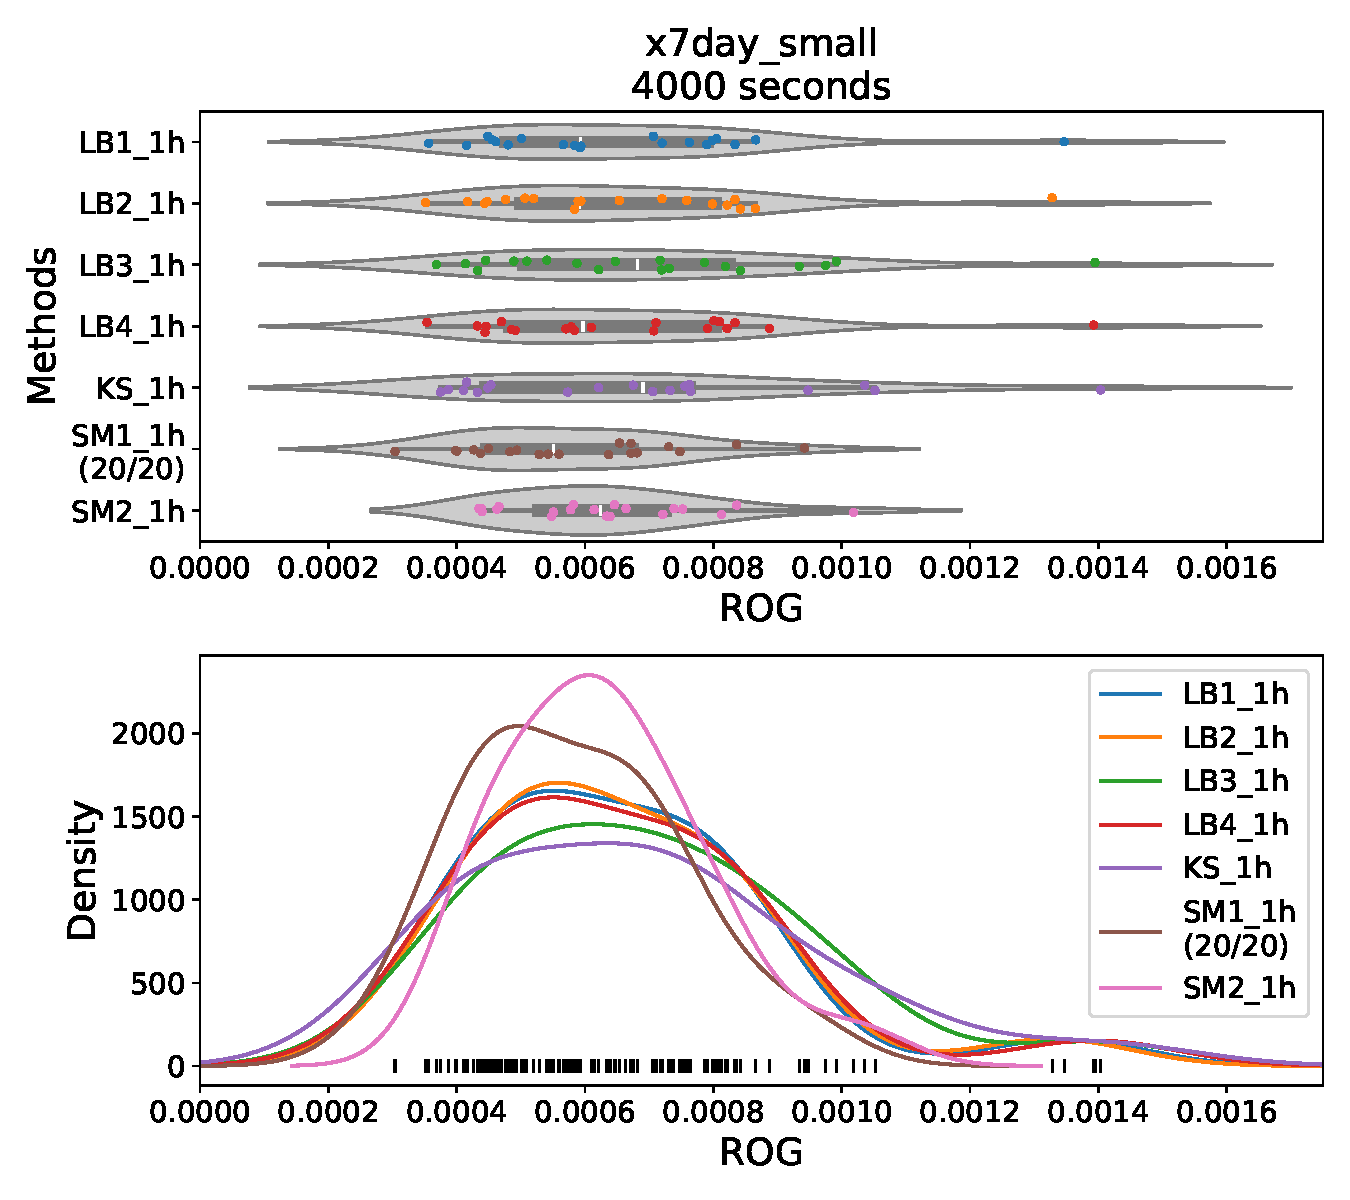
\includegraphics[width=\textwidth]{Figure/fig_violinAll_1h_x7day_small.pdf}
         \caption{Time limit of 4000 seconds}
         \label{fig_violinAll_1h_x7day_small}
     \end{subfigure}
     \hfill
     \begin{subfigure}[b]{0.48\textwidth}
         \centering
         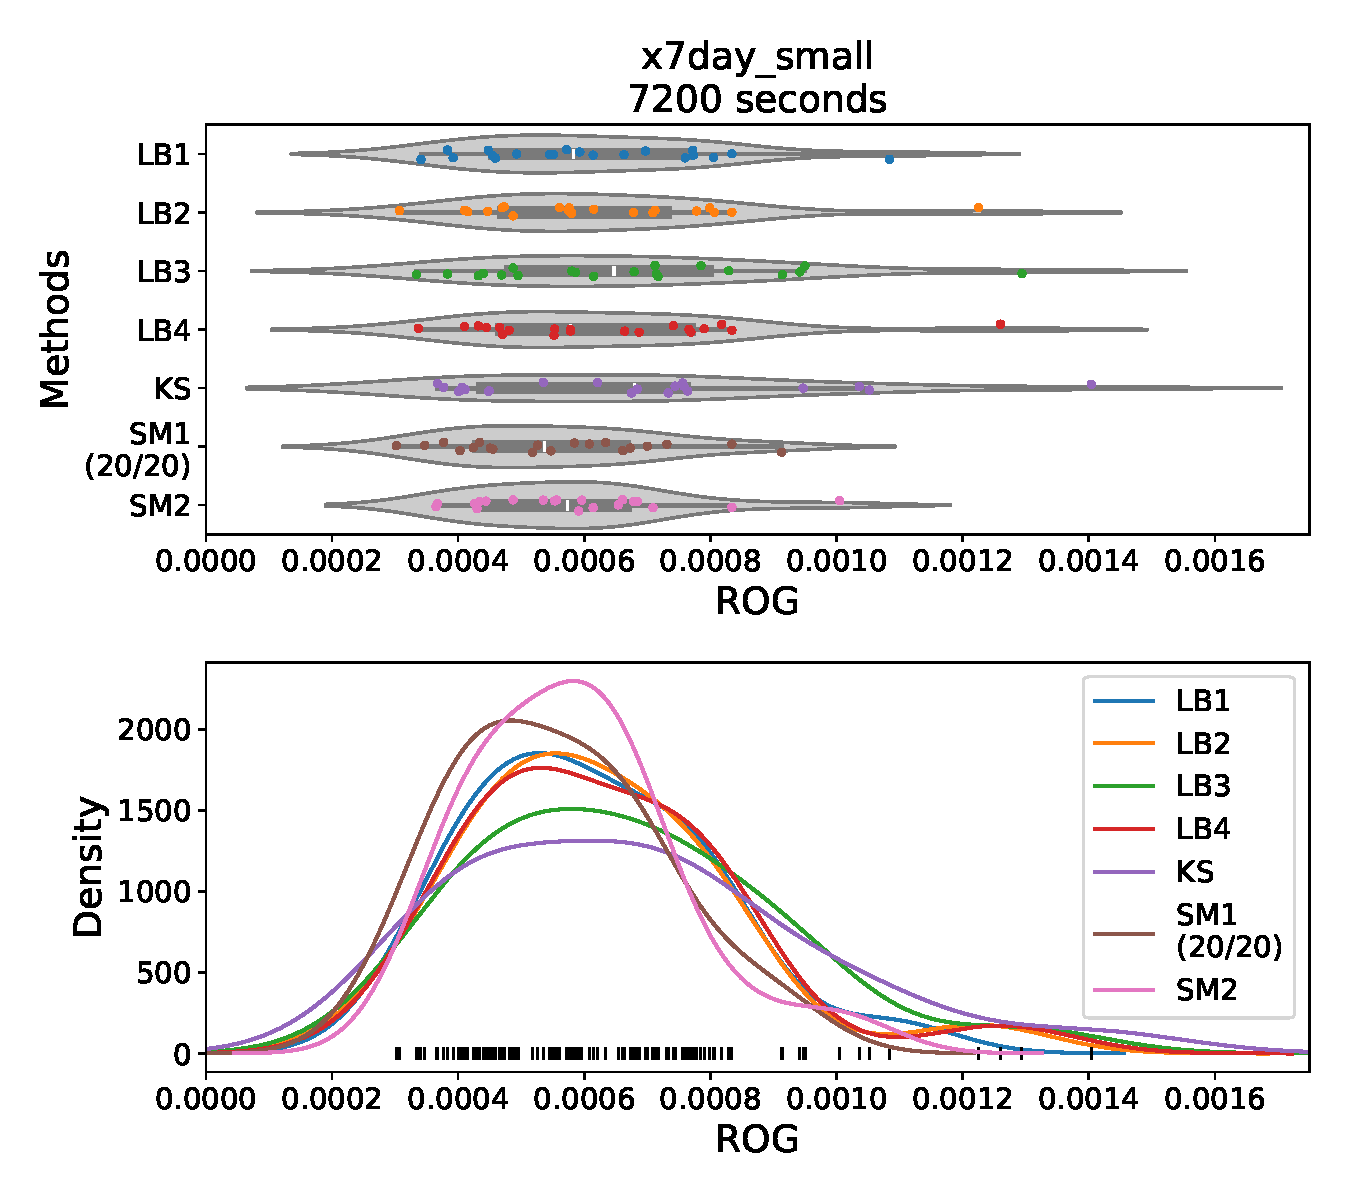
\includegraphics[width=\textwidth]{Figure/fig_violinAll_x7day_small.pdf}
         \caption{Time limit of 7200 seconds}
         \label{fig_violinAll_2h_x7day_small}
     \end{subfigure}
     \caption{Relative optimality gap distribution of improvement methods on set x7day\_small.}
\end{figure}



%%%%%%%%%%%%%%%%%%%%%%%%%%%%%%%%%%%%%%%% x7day_medium 
\begin{figure}[htpb]
     \centering
     \begin{subfigure}[b]{0.485\textwidth}
         \centering
         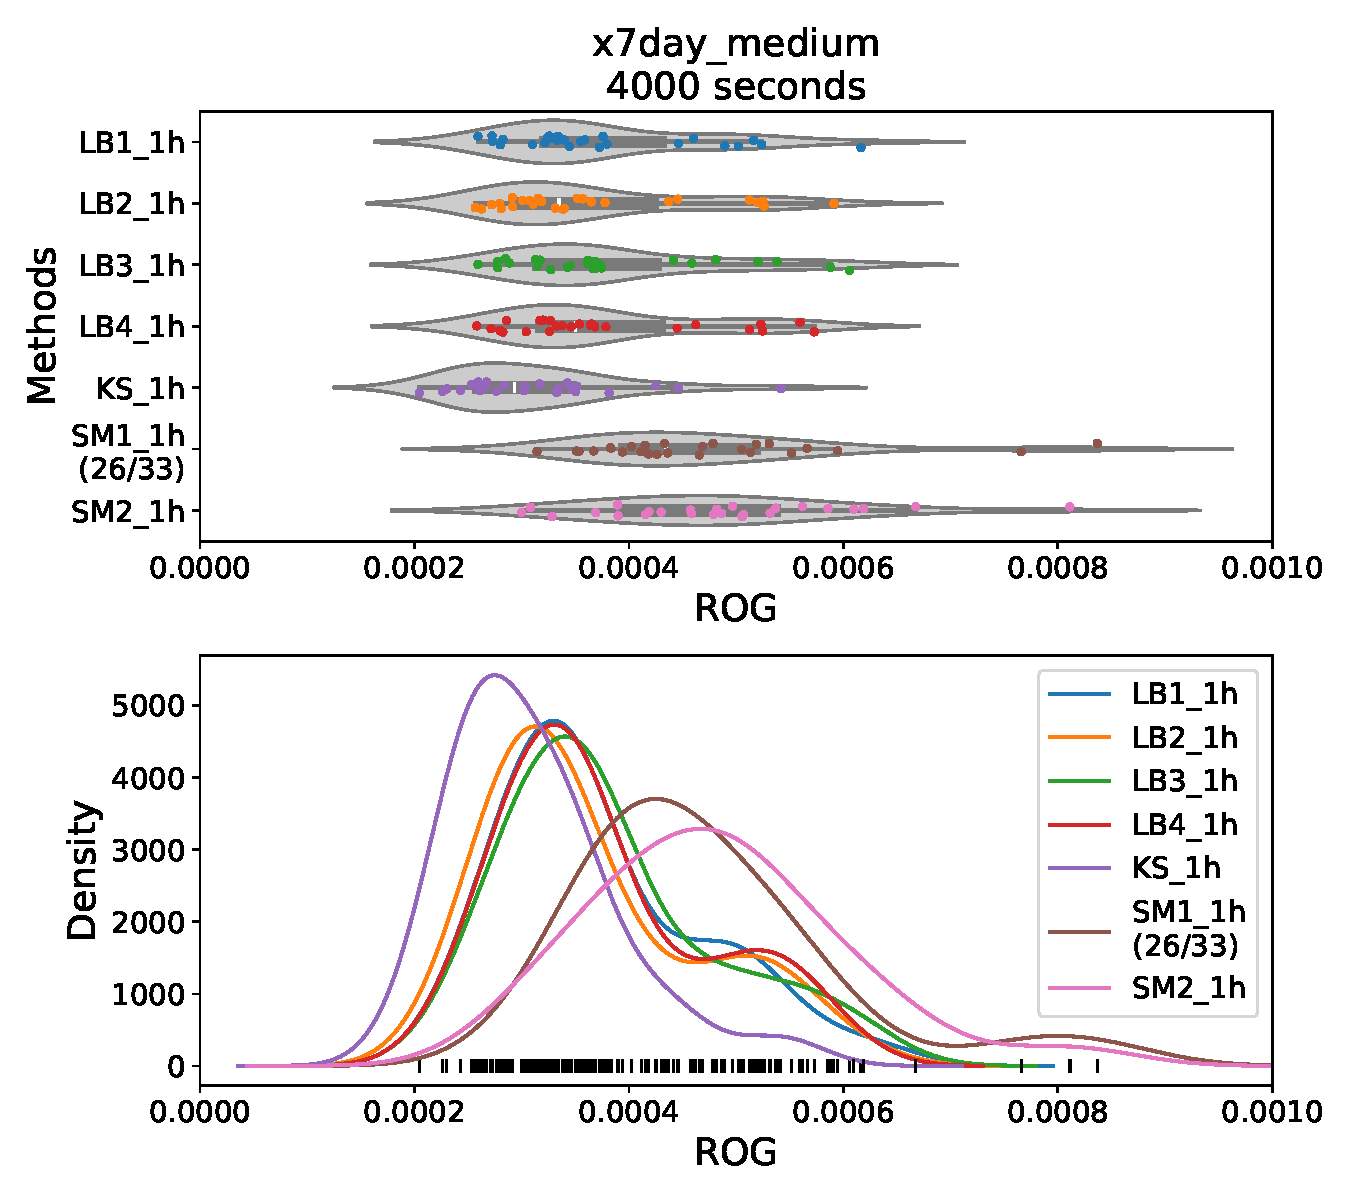
\includegraphics[width=\textwidth]{Figure/fig_violinAll_1h_x7day_medium.pdf}
         \caption{Time limit of 4000 seconds}
         \label{fig_violinAll_1h_x7day_medium}
     \end{subfigure}
     \hfill
     \begin{subfigure}[b]{0.485\textwidth}
         \centering
         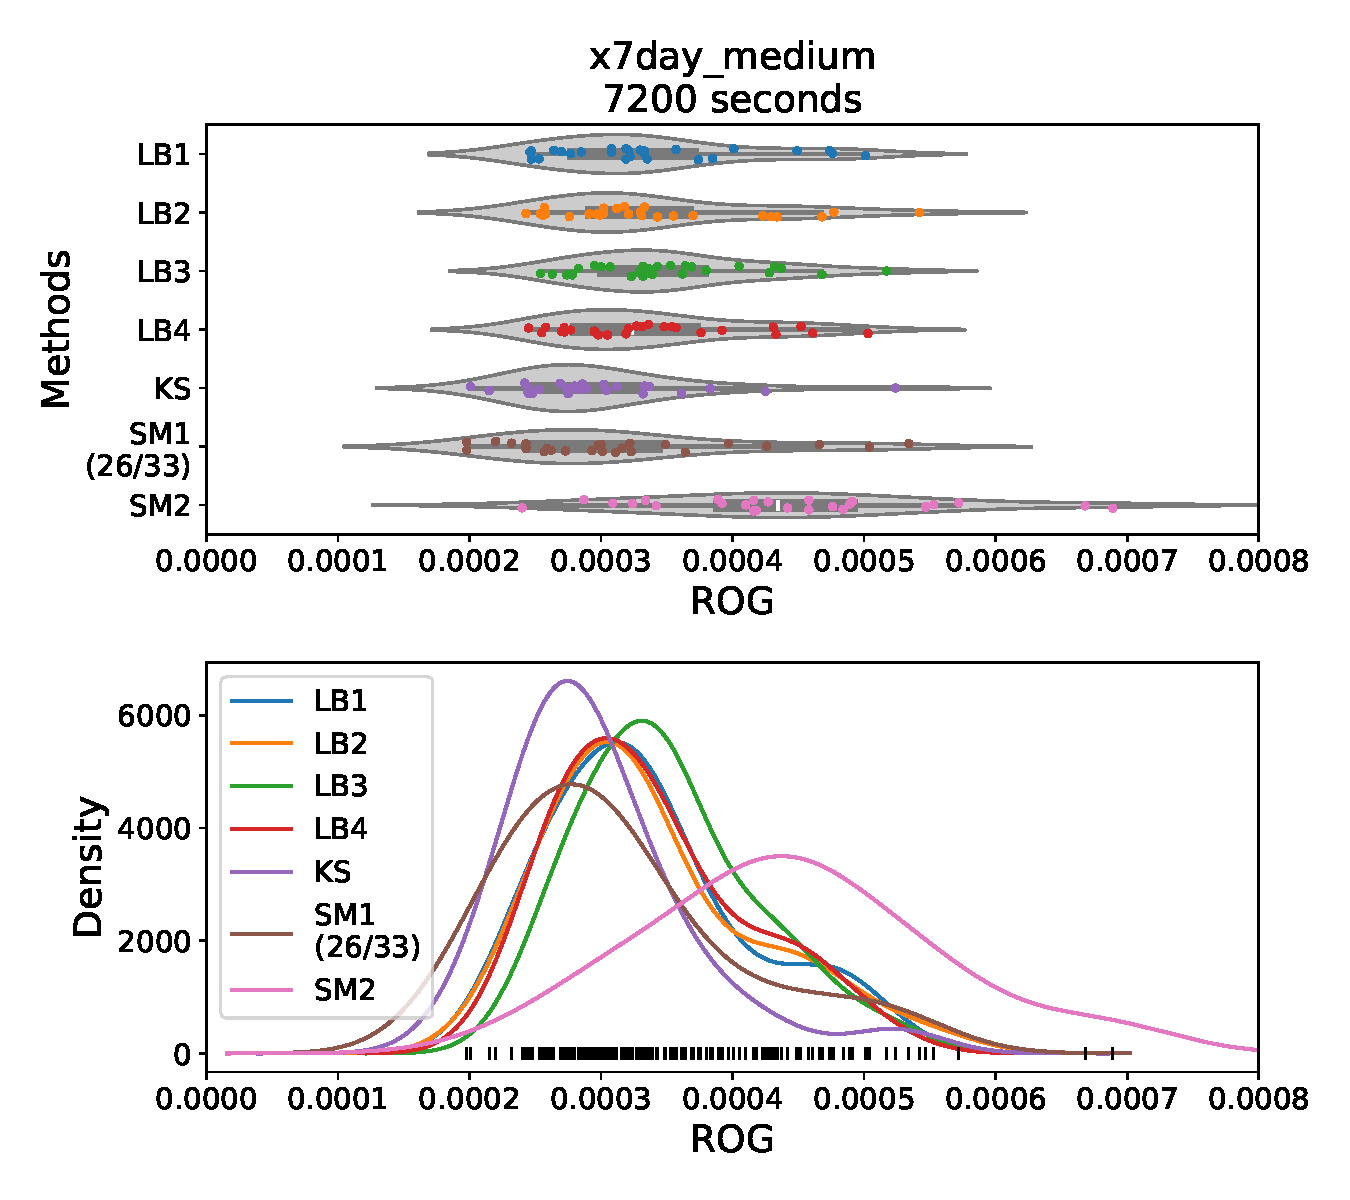
\includegraphics[width=\textwidth]{Figure/fig_violinAll_x7day_medium.pdf}
         \caption{Time limit of 7200 seconds}
         \label{fig_violinAll_2h_x7day_medium}
     \end{subfigure}
     \caption{Relative optimality gap distribution of improvement methods on set x7day\_medium.}
\end{figure}

%%%%%%%%%%%%%%%%%%%%%%%%%%%%%%%%%%%%%%%%%%%%%% x7day_large 
\begin{figure}[htb]
     \centering
     \begin{subfigure}[b]{0.48\textwidth}
         \centering
         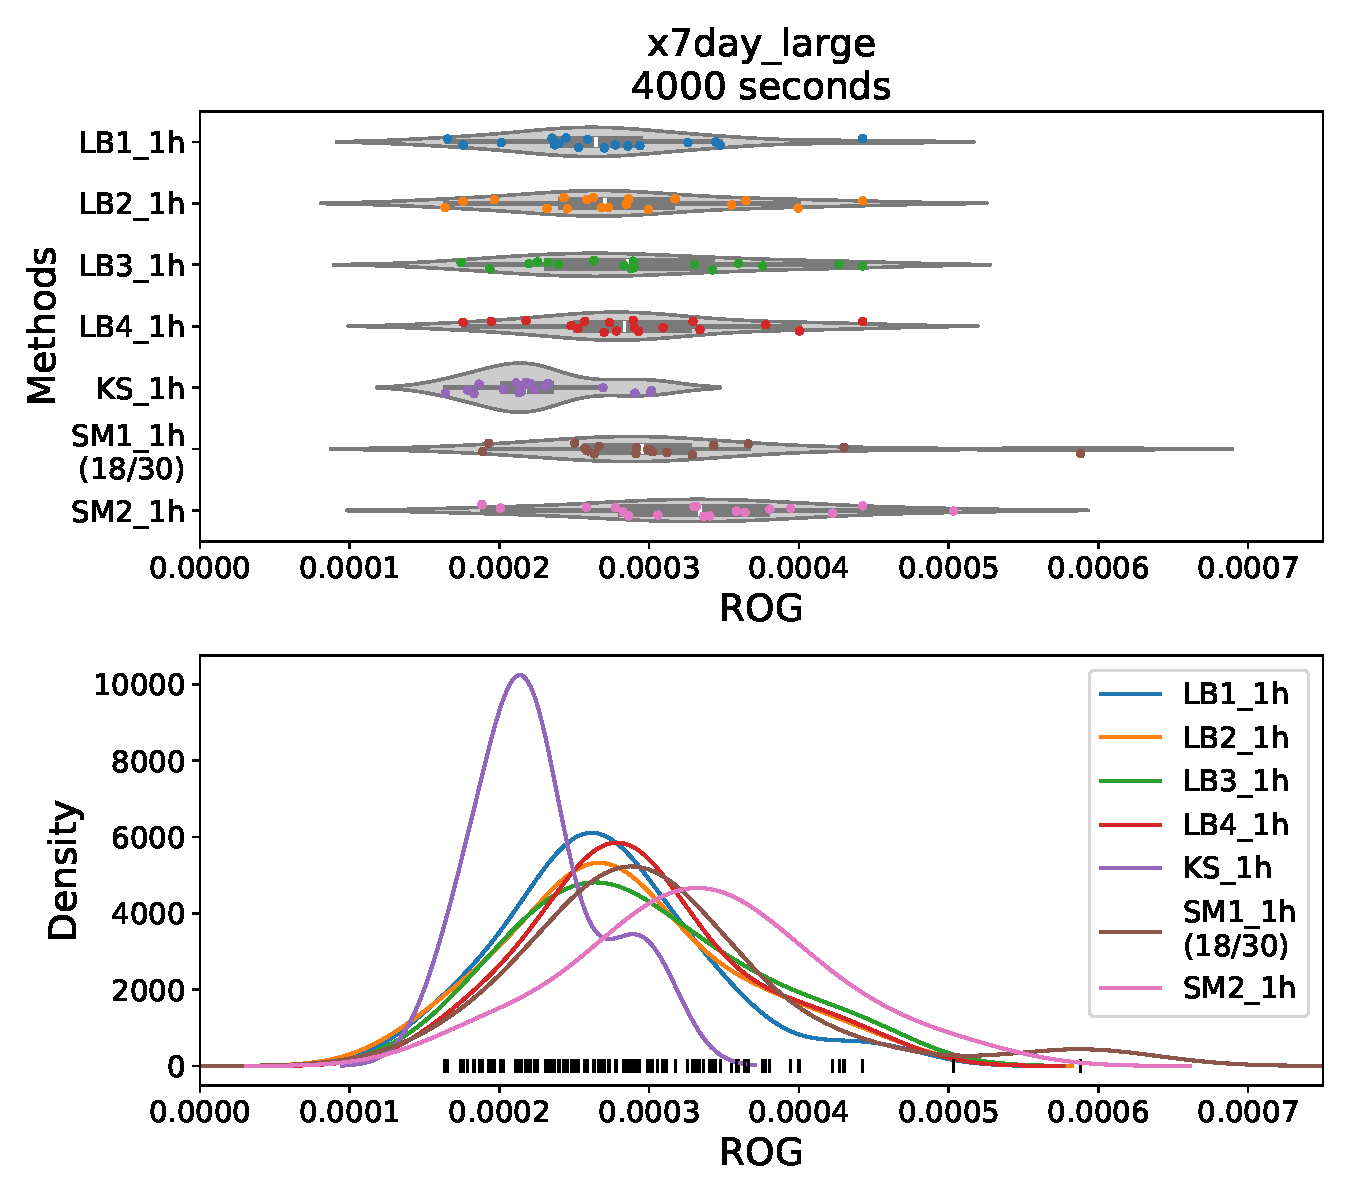
\includegraphics[width=\textwidth]{Figure/fig_violinAll_1h_x7day_large.pdf}
         \caption{Time limit of 4000 seconds}
         \label{fig_violinAll_1h_x7day_large}
     \end{subfigure}
     \hfill
     \begin{subfigure}[b]{0.48\textwidth}
         \centering
         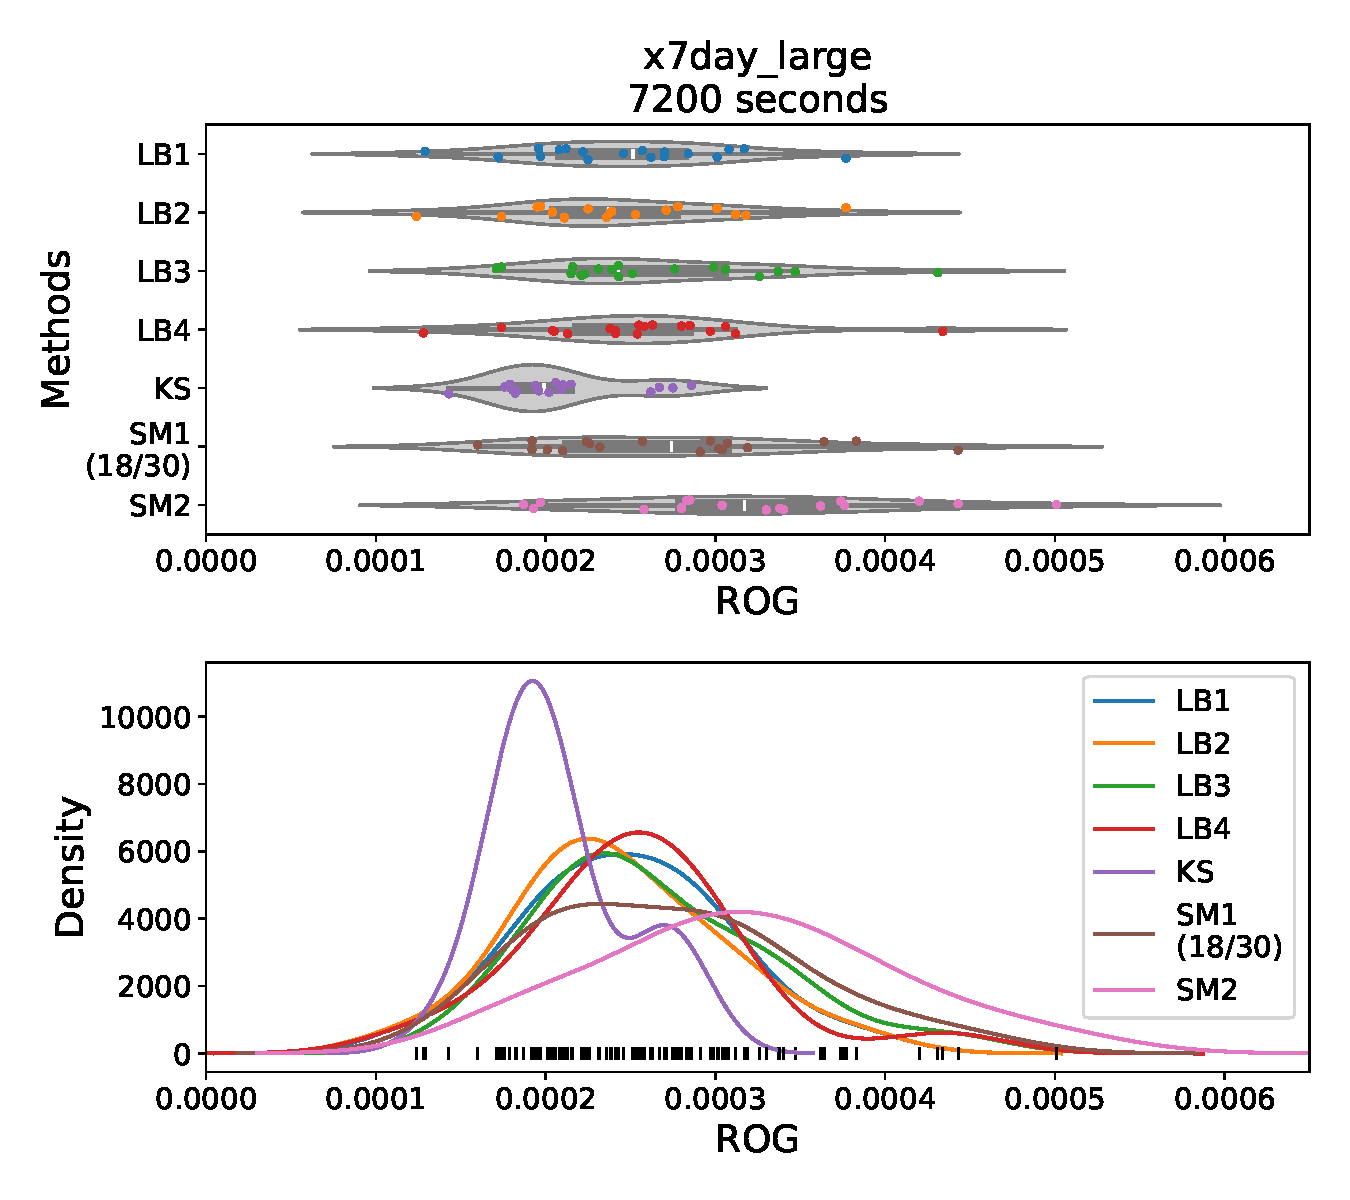
\includegraphics[width=\textwidth]{Figure/fig_violinAll_x7day_large.pdf}
         \caption{Time limit of 7200 seconds}
         \label{fig_violinAll_2h_x7day_large}
     \end{subfigure}
     \caption{Relative optimality gap distribution of improvement methods on set  x7day\_large.}
\end{figure}

\clearpage
